\chapter{Complex Numbers and the Complex Plane} % 复数与复平面
\section{Complex Numbers and Their Geometric Representation} % 复数及其几何表示
\begin{leftbarTitle}{Complex Numbers Field}\end{leftbarTitle} % 复数域
The numbers with the form \(z = x + y\mathrm{i}\), where \(x, y \in \mathbb{R}\) and \(i\) is 
the imaginary unit satisfying \(\mathrm{i}^2 = -1\), are called \textbf{complex numbers}.
\(x, y\) are called the real and imaginary parts of \(z\) with the notation \(x = \Re(z)\) (\(\mathrm{Re}(z)\)) 
and \(y = \Im(z)\) (\(\mathrm{Im}(z)\)), respectively.
When \(y = 0\), \(z\) is called a \textbf{real number}, and when \(x = 0\), \(z\) is called a \textbf{pure imaginary number}.

Complex numbers can be represented as points in the Cartesian coordinate system 
(\textbf{complex plane}, also known as the Argand plane~\ref{fig:complex_plane}), 
where the horizontal axis (the real axis) represents the real part and 
the vertical axis (the imaginary axis) represents the imaginary part.

\begin{figure}[h]
    \centering
    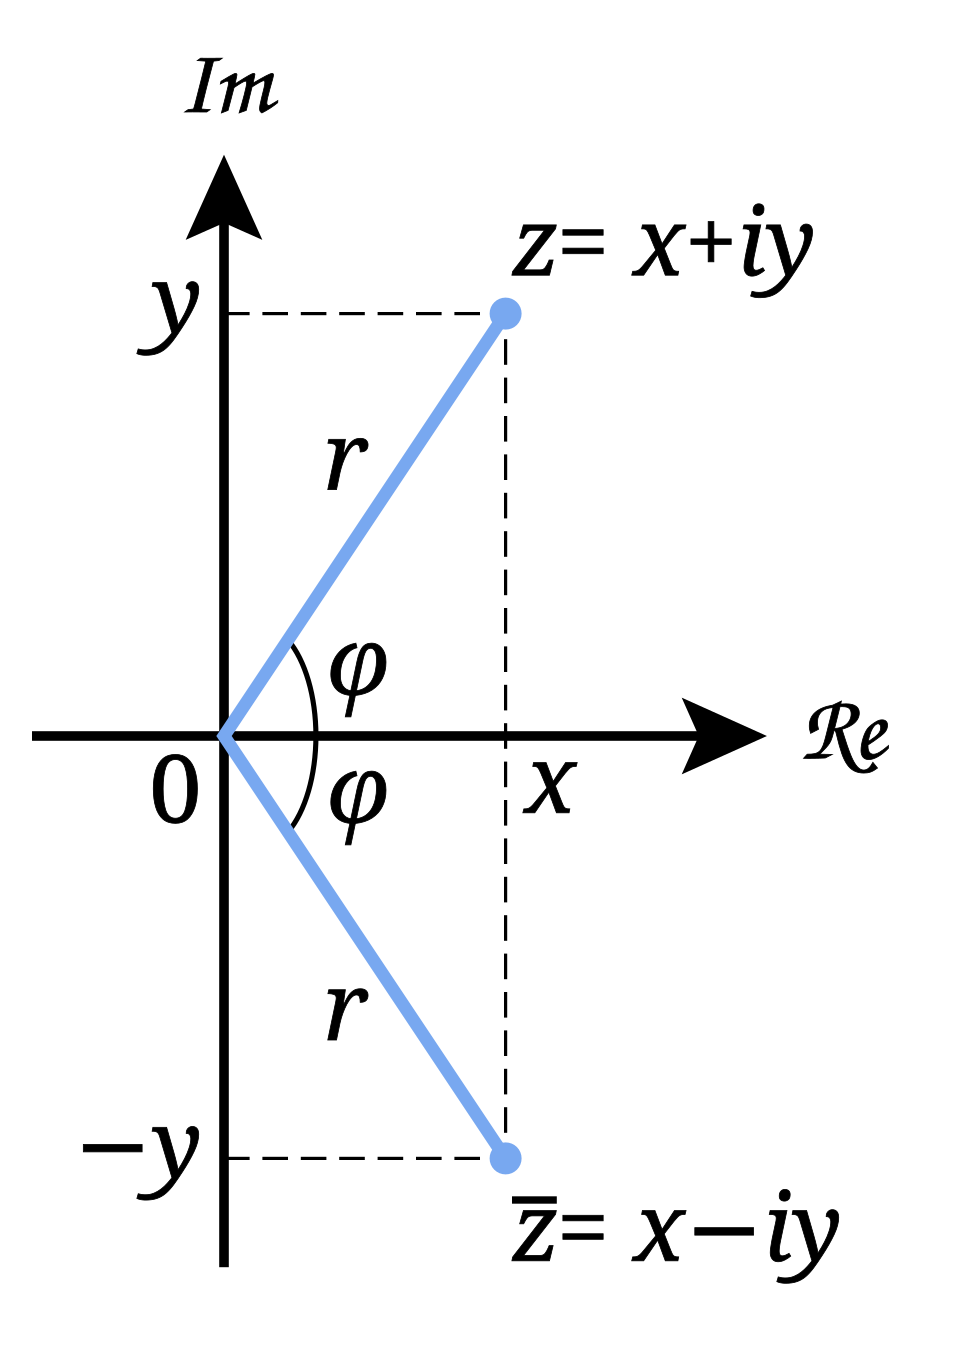
\includegraphics[width=0.25\textwidth]{img/Complex_conjugate_picture.svg.png}
    \caption{Complex number \(z\) and its conjugate \(\bar{z}\) in the complex plane.}
    \label{fig:complex_plane}
\end{figure}

\(\bar{z}=x-y\mathrm{i}\) is called the \textbf{complex conjugate} of \(z\).
It is easy to verify the following properties of complex conjugation:
\begin{enumerate}
    \item \(\overline{(\bar{z})}=z, \overline{z_{1}\pm z_{2}}=\overline{z_{1}}\pm \overline{z_{2}}\); 
    \item \(\overline{z_{1} z_{2}}=\overline{z_{1}} \cdot \overline{z_{2}}, 
    \overline{\left(\frac{z_{1}}{z_{2}}\right)}=\frac{\overline{z_{1}}}{\overline{z_{2}}}\);
    \item \(z^{2} = z\bar{z},\mathrm{Re}(z) = \frac{z + \bar{z}}{2}, \mathrm{Im}(z) = \frac{z - \bar{z}}{2\mathrm{i}}\);
    \item \(\overline{R(a, b, c, \cdots)} = R(\overline{a}, \overline{b}, \overline{c}, \cdots)\),
        where \(R\) is any rational function of its arguments.
\end{enumerate}

The set of all complex numbers is denoted by \(\mathbb{C}\).

\vspace{0.7cm}
Field is a set \(\mathbb{F}\) equipped with two operations (addition and multiplication) that satisfy:
\begin{enumerate}
    \item \((\mathbb{F}, +)\) is an abelian group.
    \item \((\mathbb{F} \setminus \{0\}, \cdot)\) is an abelian group.
    \item Multiplication is distributive over addition.
\end{enumerate}
If we define addition and multiplication of complex numbers as follows:
\[
    (x_1 + y_1\mathrm{i}) + (x_2 + y_2\mathrm{i}) = (x_1 + x_2) + (y_1 + y_2)\mathrm{i},
\]
\[
    (x_1 + y_1\mathrm{i}) \cdot (x_2 + y_2\mathrm{i}) = (x_1 x_2 - y_1 y_2) + (x_1 y_2 + x_2 y_1)\mathrm{i},
\]
then \(\mathbb{C}\) forms a field, 
% 是实数域的二次扩域, 也是特征为零的代数闭域
which is a quadratic extension of the real numbers and an algebraically closed field of characteristic zero.

% 下面我们给出几种复数域的严格定义, 以便后续的分析
Now we give several rigorous definitions of the complex number field for subsequent analysis.
\begin{definition}{Complex Numbers Field}
    \begin{description}
        % 解析/有序对定义
        \item[Analytic/Ordered Pair Definition] Let
            \[
            \mathbb{C} = \{(x, y) | x, y \in \mathbb{R}\},
            \]
            and define addition and multiplication as follows:
            \[
                (x_1, y_1) + (x_2, y_2) = (x_1 + x_2, y_1 + y_2),
            \]
            \[
                (x_1, y_1) \cdot (x_2, y_2) = (x_1 x_2 - y_1 y_2, x_1 y_2 + x_2 y_1).
            \]
            Then \((\mathbb{C}, +, \cdot)\) is a field, called the complex field.
        % 多项式商环定义
        \item[Polynomial Quotient Ring Definition] The quotient ring of the polynomial ring \(\mathbb{R}[x]\) 
            by the ideal generated by \(x^2 + 1\) is a field, denoted by 
            \[
            \mathbb{C} = \mathbb{R}[x]/(x^2 + 1),
            \]
            called the complex field.
        % 实矩阵定义
        \item[Real Matrix Definition] Let
            \[
            \mathbb{C} = \left\{\begin{pmatrix} x & -y \\ y & x \end{pmatrix} | x, y \in \mathbb{R}\right\}.
            \]
            Then \((\mathbb{C}, +, \cdot)\) is a field, 
            where addition and multiplication are defined as matrix addition and multiplication, respectively, 
            called the complex field.
    \end{description}
\end{definition}
% 由于域保证了非零元素的乘法逆元存在, 因此我们可以定义复数的除法
Since the field guarantees the existence of multiplicative inverses for non-zero elements,
we can define the division of complex numbers as follows:
\[
    z^{-1} = \frac{1}{z} = \frac{\bar{z}}{|z|^2} = \frac{x - y\mathrm{i}}{x^2 + y^2}.
\]

\begin{leftbarTitle}{Other Representations of Complex Numbers}\end{leftbarTitle} % 复数的其他表示
For a non-zero complex number \(z=x+y\mathrm{i}\), the \textbf{argument} of \(z\),
denoted by \(\mathrm{Arg}(z)=\tan^{-1}\left(\frac{y}{x}\right)\), is defined as 
the angle \(\varphi\) between the positive real axis and the line segment from the origin to the point \(z\) in the complex plane, 
measured in the counterclockwise direction.
% 显然一个复数对应无数个辐角, 因此我们通常定义主值 \(\arg(z)\) 来表示在 \((-\pi, \pi]\) 范围内的唯一一个辐角
It's obvious that a complex number corresponds to infinitely many arguments, 
so we usually define the principal value \(\arg(z)\) to represent the unique argument in the range \((-\pi, \pi]\).

Moreover, we define the \textbf{modulus} of \(z\) as \(r = |z| = \sqrt{x^2 + y^2}\), 
which is the distance from the origin to the point \(z\) in the complex plane.
Then we can express \(z\) in polar form as
\[
    z = r(\cos \varphi + \mathrm{i} \sin \varphi) = r e^{\mathrm{i} \varphi},
\]
where \(e^{\mathrm{i} \varphi} = \cos \varphi + \mathrm{i} \sin \varphi\) is known as \textbf{Euler's formula}
(refer to Fig.~\ref{fig:complex_plane}).

% 复数的极坐标表示使得我们可以方便地进行乘法和除法运算, 因为它们对应于模长的乘积和商以及辐角的和与差
The polar representation of complex numbers allows us to conveniently perform multiplication and division,
as they correspond to the product and quotient of moduli and the sum and difference of arguments, respectively:
\[
    z_1 z_2 = r_1 r_2 e^{\mathrm{i} (\varphi_1 + \varphi_2)}, \quad
    \frac{z_1}{z_2} = \frac{r_1}{r_2} e^{\mathrm{i} (\varphi_1 - \varphi_2)}.
\]
% 并且据此我们知道两个复数做乘法就相当于模长相乘, 辐角相加; 做除法就相当于模长相除, 辐角相减
Thus, we know that \emph{multiplying two complex numbers is equivalent to multiplying their moduli and adding their arguments, 
while dividing two complex numbers is equivalent to dividing their moduli and subtracting their arguments}.

\begin{remark}
    % 借助复数的极坐标表示, 我们可以很容易地证明一些三角恒等式, 例如倍角公式和和差公式
    With the help of the polar representation of complex numbers, we can easily prove some trigonometric identities,
    such as the double-angle formulas and the sum and difference formulas.
    For example, using Euler's formula, we have
    \[
        e^{\mathrm{i} 2\varphi} = (e^{\mathrm{i} \varphi})^2 = (\cos \varphi + \mathrm{i} \sin \varphi)^2 = \cos 2\varphi + \mathrm{i} \sin 2\varphi,
    \]
    which gives us the double-angle formulas:
    \[
        \cos 2\varphi = 2\cos^2 \varphi - 1, \quad
        \sin 2\varphi = 2\sin \varphi \cos \varphi.
    \]
    Similarly, we can derive the sum and difference formulas for sine and cosine.
\end{remark}

\begin{remark}
    % 借助复数的极坐标表示, 我们可以重写复数域的实矩阵定义, 以便更好地理解复数的几何意义
    With the help of the polar representation of complex numbers, we can rewrite the real matrix definition of the complex field
    to better understand the geometric meaning of complex numbers:
    
    ``Let
    \[
    \mathbb{C} = \left\{\begin{pmatrix} r\cos \varphi & -r\sin \varphi \\ r\sin \varphi & r\cos \varphi \end{pmatrix} | r \geq 0, \varphi \in [0, 2\pi) \right\}.
    \]
    Then we can verify that the addition and multiplication defined as matrix addition and multiplication, respectively, 
    are consistent with the polar representation of complex numbers.''

    % 当模长为 1 时, 这就是解析几何中的旋转矩阵, 它表示了复数在复平面上的旋转作用
    When the modulus is \(1\), this is the rotation matrix in analytic geometry, 
    which represents the rotational effect of complex numbers in the complex plane.
\end{remark}

\begin{leftbarTitle}{Powers and Roots of Complex Numbers}\end{leftbarTitle} % 复数的幂与根
Let \(z = r e^{\mathrm{i} \varphi}\) be a non-zero complex number. 
For any integer \(n\), we have
\[
    z^n = r^n e^{\mathrm{i} n \varphi} = r^n (\cos n\varphi + \mathrm{i} \sin n\varphi).
\]
Then it can be derived that
\[
    \left| z^{n} \right| = r^{n}, \quad \mathrm{Arg}(z^{n}) = n \varphi.
\]
When \(r=1\), it is called \textbf{De Moivre's formula}:
\[
(\cos \varphi + \mathrm{i} \sin \varphi)^n = \cos n\varphi + \mathrm{i} \sin n\varphi.
\]

Find the \(n\)-th roots of \(z\) is equivalent to solving the equation \(\omega^n = z\),
which has \(n\) distinct solutions given by
\[
    \omega_k = r^{\frac{1}{n}} e^{\mathrm{i} \left(\frac{\varphi + 2k\pi}{n}\right)} = r^{\frac{1}{n}} \left[\cos \left(\frac{\varphi + 2k\pi}{n}\right) + \mathrm{i} \sin \left(\frac{\varphi + 2k\pi}{n}\right)\right], \quad k = 0, 1, \ldots, n-1.
\]
\section{The Extended Complex Plane} % 扩充复平面

The \textbf{extended complex plane}, denoted by \(\hat{\mathbb{C}}\), 
is defined as the union of the complex plane \(\mathbb{C}\) and the point at infinity \(\infty\):
\[
    \hat{\mathbb{C}} = \mathbb{C} \cup \{\infty\}.
\]
This extension allows us to treat infinity as a point in the complex plane,
which is particularly useful in complex analysis for 
studying the behavior of functions at infinity and for compactifying the complex plane.

The extended complex plane can be visualized as a sphere, called the \textbf{Riemann sphere}, 
where the point at infinity corresponds to the north pole of the sphere.
\begin{figure}[h]
    \centering
    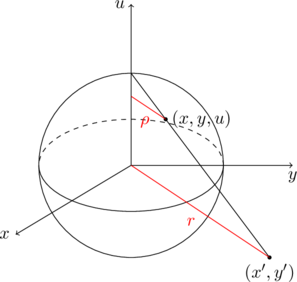
\includegraphics[width=0.4\textwidth]{img/extended_complex_plane.png}
    \caption{The extended complex plane, also known as the Riemann sphere.}
    \label{fig:extended_complex_plane}
\end{figure}
% 在扩充复平面上, 每条直线都通过无穷远点相交, 因此我们可以将扩充复平面看作是一个紧致化的复平面
In the extended complex plane, every line intersects at the point at infinity,
so we can view the extended complex plane as a compactification of the complex plane.
This compactification allows us to apply topological and geometric methods to study complex functions,
especially those that have singularities or poles at infinity.